% Manual de uso de FisGraf, FisErr y fisgraf-cli.
% Compilar con: manual/compilar.bat  (o: latexmk -lualatex manual.tex)
% Si antes se define \SoloFisErr, sale el manual reducido de FisErr
% (lo usa compilar.bat para crear manual_fiserr.pdf).
\documentclass[11pt,a4paper]{article}
\newif\iffiserr
\ifdefined\SoloFisErr \fiserrtrue \fi
% Si se define \Portable, sale el manual de la carpeta portable: sin fisgraf-cli
% ni Claude, y con las rutas de esa carpeta (manual_portable.tex).
\newif\ifportable
\ifdefined\Portable \portabletrue \fi

\usepackage{fontspec}
\usepackage[spanish,es-noshorthands]{babel}
\usepackage{amsmath,amssymb}
\usepackage[a4paper,margin=2.2cm,headheight=14pt]{geometry}
\usepackage{xcolor}
\usepackage{graphicx}
\usepackage{tabularx,booktabs,array}
\usepackage{enumitem}
\usepackage{fancyhdr}
\usepackage{titlesec}
\usepackage[most]{tcolorbox}
\usepackage{listings}
\usepackage{siunitx}
\usepackage{tikz}
\usetikzlibrary{positioning}
\usepackage[hidelinks]{hyperref}

\definecolor{azul}{HTML}{14213D}
\definecolor{azul2}{HTML}{1F3A63}
\definecolor{naranja}{HTML}{FCA311}
\definecolor{verde}{HTML}{17606B}
\definecolor{gris}{HTML}{F2F2F2}
\definecolor{texto2}{HTML}{555555}

\sisetup{output-decimal-marker={,}}
\setlist{itemsep=2pt,topsep=4pt}
\setlength{\parindent}{0pt}
\setlength{\parskip}{5pt}
\renewcommand{\arraystretch}{1.25}
% Margen para párrafos con muchas palabras en monoespaciada (no se dividen).
\setlength{\emergencystretch}{3em}

% Títulos con el color de cada aplicación.
\titleformat{\section}{\Large\bfseries\color{azul}}{\thesection}{0.6em}{}[{\color{naranja}\titlerule[1.2pt]}]
\titleformat{\subsection}{\large\bfseries\color{azul2}}{\thesubsection}{0.6em}{}
\titlespacing*{\section}{0pt}{16pt}{8pt}
\titlespacing*{\subsection}{0pt}{12pt}{4pt}

\pagestyle{fancy}
\fancyhf{}
\iffiserr
  \fancyhead[L]{\small\color{texto2}Manual de uso · FisErr}
\else\ifportable
  \fancyhead[L]{\small\color{texto2}Manual de uso · FisGraf y FisErr}
\else
  \fancyhead[L]{\small\color{texto2}Manual de uso · FisGraf, FisErr y fisgraf-cli}
\fi\fi
% Filas de tabla que solo van en el manual completo (un \if no puede cruzar un &).
\ifportable
  \newcommand{\filacli}{}
  \newcommand{\filarust}{}
\else
  \newcommand{\filacli}{\textbf{fisgraf-cli} & Las mismas funciones por línea de comandos y como servidor MCP para IA.\\}
  \newcommand{\filarust}{\textbf{Rust} & Solo para compilar los programas (crear o actualizar los \code{.exe}).\\}
\fi
\fancyhead[R]{\small\color{texto2}\leftmark}
\fancyfoot[C]{\small\thepage}
\renewcommand{\headrulewidth}{0.4pt}
\renewcommand{\sectionmark}[1]{\markboth{#1}{}}

% Recuadros.
\newtcolorbox{nota}[1][Nota]{colback=gris,colframe=verde,fonttitle=\bfseries,title=#1,boxrule=0.6pt,arc=2pt,left=6pt,right=6pt}
\newtcolorbox{consejo}{colback=naranja!8,colframe=naranja,boxrule=0.6pt,arc=2pt,left=6pt,right=6pt,before upper={\textbf{Consejo.}\ }}

% Código.
\newcommand{\code}[1]{\texttt{#1}}
\newcommand{\bs}{\textbackslash}
\newcommand{\boton}[1]{\textsf{\bfseries #1}}
\newcommand{\menu}[1]{\textsf{#1}}
\lstset{basicstyle=\ttfamily\small,backgroundcolor=\color{gris},frame=single,rulecolor=\color{verde!50},
  framesep=4pt,xleftmargin=6pt,xrightmargin=6pt,columns=fullflexible,keepspaces=true,showstringspaces=false,breaklines=true}

% Subtítulo dentro de una sección (en bloque, no en línea como \paragraph).
\newcommand{\bloque}[1]{\par\medskip{\bfseries\color{azul2}#1}\par\nopagebreak\smallskip}

% Tabla de opciones: nombre a la izquierda, descripción alineada a la izquierda.
\newenvironment{opciones}{\par\noindent\tabularx{\linewidth}{@{}>{\raggedright\arraybackslash}p{0.30\linewidth}>{\raggedright\arraybackslash}X@{}}\toprule
  \textbf{Opción} & \textbf{Qué hace}\\\midrule}{\bottomrule\endtabularx\par}

\begin{document}

% ------------------------------------------------------------------ Portada
\iffiserr
\begin{titlepage}
  \centering
  \vspace*{2.5cm}
  
\includegraphics[width=3.8cm]{../errores/assets/logo.png}\par
  \vspace{1.5cm}
  {\Huge\bfseries\color{azul} Manual de uso\par}
  \vspace{0.4cm}
  {\Large FisErr\par}
  \vspace{0.3cm}
  {\color{naranja}\rule{0.55\linewidth}{1.5pt}\par}
  \vspace{0.6cm}
  {\large Calculadora de propagación de errores:\\ el valor final con su error y la función del error\par}
  \vfill
\end{titlepage}
\else
\begin{titlepage}
  \centering
  \vspace*{2.5cm}
  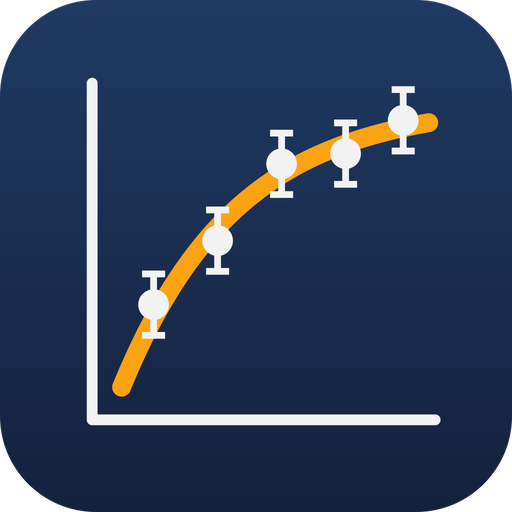
\includegraphics[width=3.4cm]{../graficos/assets/logo.png}\hspace{1.2cm}%
  
\includegraphics[width=3.4cm]{../errores/assets/logo.png}\par
  \vspace{1.5cm}
  {\Huge\bfseries\color{azul} Manual de uso\par}
  \vspace{0.4cm}
  {\Large FisGraf · FisErr\ifportable\else{} · fisgraf-cli\fi\par}
  \vspace{0.3cm}
  {\color{naranja}\rule{0.55\linewidth}{1.5pt}\par}
  \vspace{0.6cm}
  {\large Gráficos de datos de física, ajustes de modelos\\ y propagación de errores con calidad LaTeX\par}
  \vfill
  \begin{tabular}{@{}l@{\quad}p{9cm}@{}}
    \textbf{\color{azul}FisGraf} & Gráficos desde Excel o CSV con ajustes, errores, $R^2$ y residuos.\\[3pt]
    \textbf{\color{verde}FisErr} & Calculadora de errores: valor final con su error y la función del error.\\[3pt]
    \filacli
  \end{tabular}
  \vspace{1.5cm}
\end{titlepage}
\fi

\tableofcontents
\newpage

% ------------------------------------------------------------------ 1
\section{Antes de empezar}

\iffiserr
\subsection{Abrir el programa}

Doble clic en \code{FisErr.exe}. No necesita instalación ni ningún otro programa: el \code{.exe} se puede copiar a cualquier carpeta, pendrive o computador con Windows 10 u 11. Para crear un acceso directo: clic derecho sobre el \code{.exe} $\rightarrow$ \menu{Enviar a} $\rightarrow$ \menu{Escritorio}.

\subsection{Convenciones}

\begin{itemize}
  \item $\sigma$ es la \emph{incertidumbre estándar}: el «error» de una medición, expresado como una desviación estándar.
  \item Las ecuaciones se escriben en \textbf{sintaxis calculable}: \code{4*pi\^{}2*L/T\^{}2} (ver sección~\ref{sec:ecuaciones}).
\end{itemize}
\else

\subsection{Requisitos}

\begin{tabularx}{\linewidth}{@{}lX@{}}\toprule
\textbf{Programa} & \textbf{Necesario para}\\\midrule
\textbf{MiKTeX} (o TeX Live) & La vista LaTeX y la exportación de gráficos en FisGraf\ifportable\else, y el comando \code{grafico} de \code{fisgraf-cli}\fi. FisErr no lo necesita.\\
\filarust\bottomrule
\end{tabularx}

\subsection{Abrir los programas}

\ifportable
\begin{tabularx}{\linewidth}{@{}lX@{}}\toprule
\textbf{Programa} & \textbf{Doble clic en}\\\midrule
FisGraf & \code{FisGraf\bs FisGraf.exe}\\
FisErr & \code{FisErr\bs FisErr.exe}\\\bottomrule
\end{tabularx}

No hay que instalar nada: la carpeta se puede copiar a un pendrive o a cualquier computador con Windows 10 u 11. Deja las carpetas \code{examples} y \code{datos\_de\_prueba} junto a \code{FisGraf.exe} para que funcionen los menús de ejemplos. Para crear un acceso directo: clic derecho sobre el \code{.exe} $\rightarrow$ \menu{Enviar a} $\rightarrow$ \menu{Escritorio}.
\else
\begin{tabularx}{\linewidth}{@{}llX@{}}\toprule
\textbf{Programa} & \textbf{Doble clic en} & \textbf{Si el \code{.exe} no existe}\\\midrule
FisGraf & \code{graficos\bs FisGraf.exe} & doble clic en \code{graficos\bs crear\_ejecutable.bat}\\
FisErr & \code{errores\bs FisErr.exe} & doble clic en \code{errores\bs crear\_ejecutable.bat}\\\bottomrule
\end{tabularx}

Para llevarlos a otro computador usa la carpeta \code{portable} (se crea con \code{crear\_portable.bat}): sus \code{.exe} no necesitan instalar nada. Para crear un acceso directo: clic derecho sobre el \code{.exe} $\rightarrow$ \menu{Enviar a} $\rightarrow$ \menu{Escritorio}.
\fi

\subsection{Convenciones}

\begin{itemize}
  \item $\sigma$ es la \emph{incertidumbre estándar}: el «error» de una medición, expresado como una desviación estándar.
  \item Todo texto que aparece en los gráficos se escribe en \textbf{LaTeX}: \code{\$T\_0\$}, \code{[\bs unit\{m/s\^{}2\}]}. Lo que no va entre \code{\$…\$} es texto normal.
  \item Las ecuaciones se escriben en \textbf{sintaxis calculable}: \code{2*pi*sqrt(L/g)} (ver sección~\ref{sec:ecuaciones}).
\end{itemize}
\fi

\iffiserr\else
% ------------------------------------------------------------------ 2
\section{FisGraf}

FisGraf toma mediciones de un Excel o un CSV, ajusta modelos teóricos, calcula el error de cada parámetro y genera un gráfico con calidad de publicación en LaTeX.

\begin{center}
  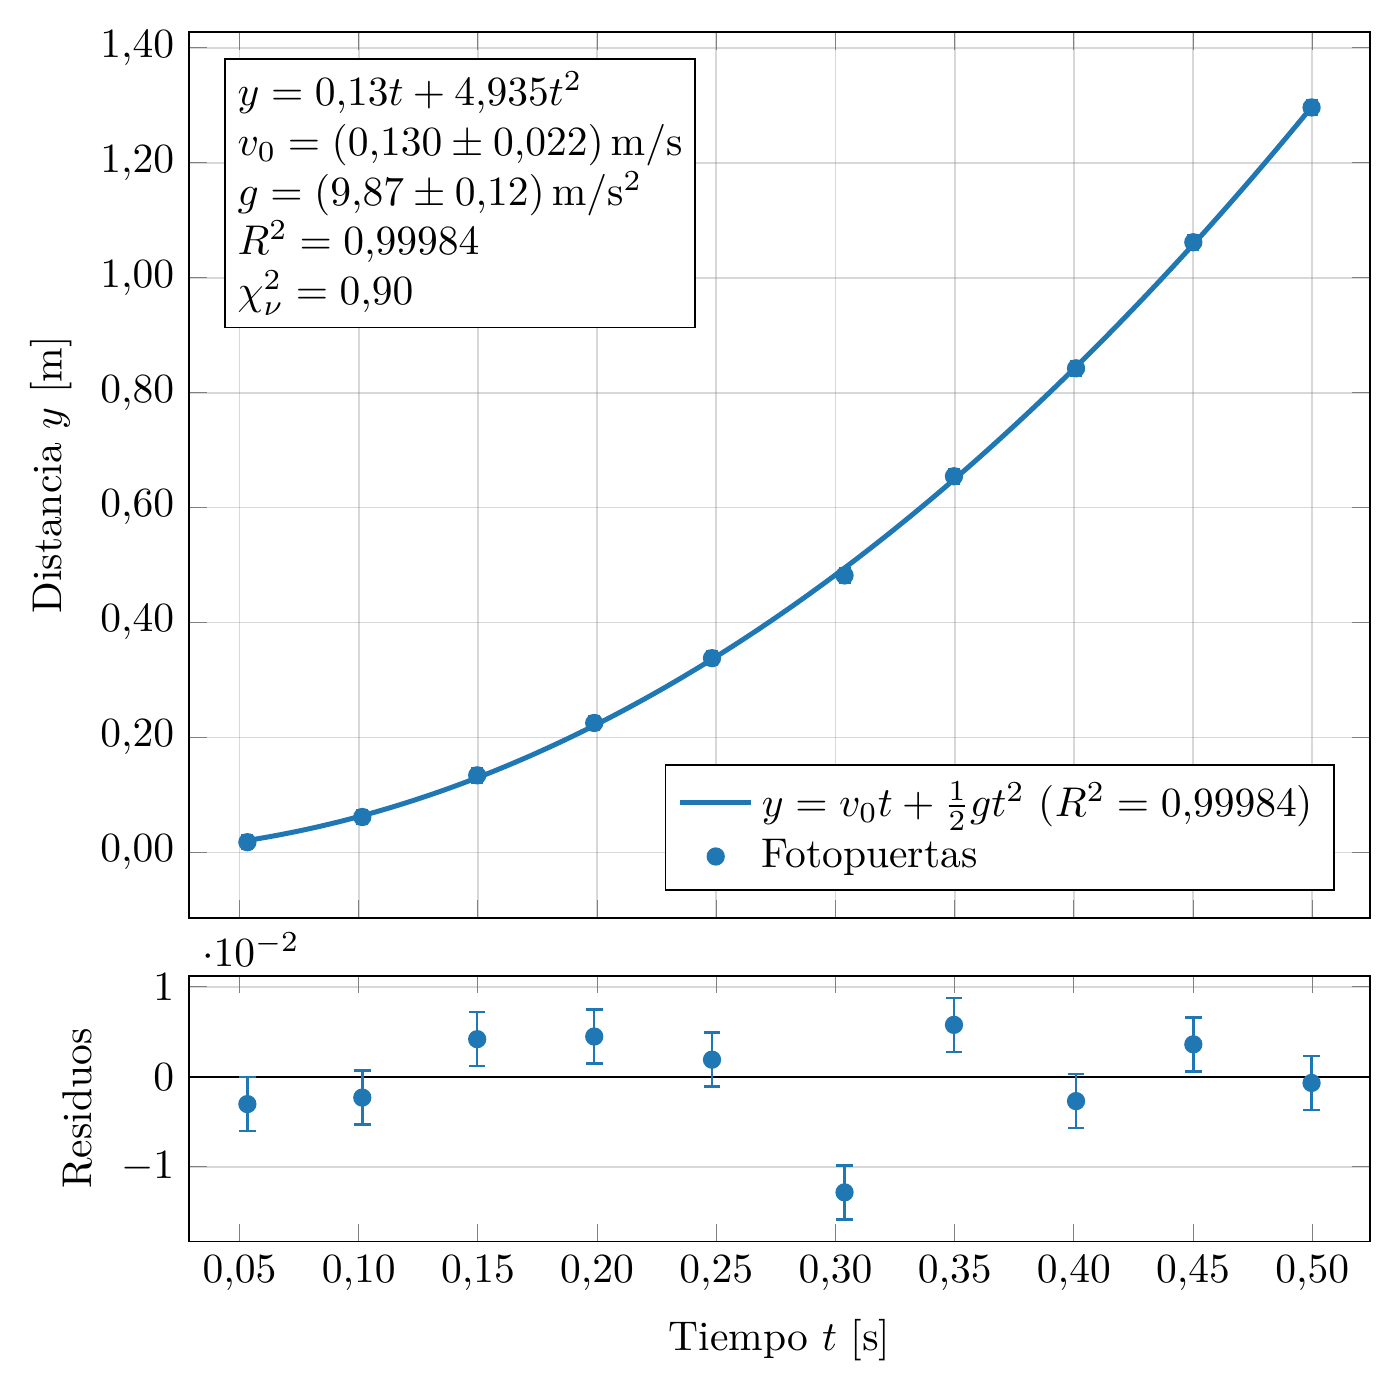
\includegraphics[width=0.62\linewidth]{../graficos/datos_de_prueba/graficos/01_caida_libre.png}\\[2pt]
  {\small\color{texto2}Ejemplo: caída libre con ajuste, ecuación ajustada, $R^2$, $\chi^2_\nu$ y residuos.}
\end{center}

\subsection{La ventana}

\begin{center}
\begin{tikzpicture}[font=\sffamily\small, every node/.style={inner sep=3pt}]
  \draw[azul, fill=azul!8, rounded corners=2pt] (0,0) rectangle (14,7.4);
  \fill[azul] (0,6.95) rectangle (14,7.4);
  \node[white, anchor=west] at (0.15,7.17) {Archivo \quad Editar};
  \node[white, anchor=east] at (13.85,7.17) {Calculado en … ms};
  % Panel izquierdo
  \draw[azul2, fill=white] (0.15,1.55) rectangle (4.3,6.8);
  \node[anchor=north west, text width=3.9cm, align=left] at (0.2,6.75)
    {\textbf{Pestañas}\\ Datos · Series · Ajustes\\ Referencias · Ejes\\ Estilo · Exportar\\ Propagación\\[6pt]\color{texto2}(opciones de la pestaña elegida)};
  % Centro
  \draw[azul2, fill=white] (4.45,1.55) rectangle (13.85,6.8);
  \node[anchor=north west] at (4.5,6.75) {\textbf{[Vista rápida]}\quad [Vista LaTeX]};
  \draw[naranja, line width=1.5pt] (5.3,2.1) .. controls (8,2.4) and (10,4.8) .. (13.2,6.0);
  \foreach \x/\y in {5.8/2.25, 7.4/2.75, 9.0/3.75, 10.6/4.85, 12.3/5.65} {\fill[azul] (\x,\y) circle (0.08);}
  \node[texto2] at (9.15,1.85) {vista previa del gráfico};
  % Inferior
  \draw[azul2, fill=white] (0.15,0.15) rectangle (13.85,1.4);
  \node[anchor=north west, text width=13.4cm, align=left] at (0.2,1.35)
    {\textbf{[Resultados] [Mensajes]}\\ \color{texto2}parámetros $\pm\,\sigma$, $R^2$, $\chi^2_\nu$, avisos…};
\end{tikzpicture}
\end{center}

\begin{itemize}
  \item \textbf{Izquierda:} las pestañas de configuración.
  \item \textbf{Centro:} la vista previa. La \boton{Vista rápida} es instantánea y aproximada. La \boton{Vista LaTeX} muestra el gráfico final compilado: tarda unos segundos y se actualiza sola.
  \item \textbf{Abajo:} \boton{Resultados}, con cada ajuste, sus parámetros, errores y estadísticos, y \boton{Mensajes}, con los avisos y errores (por ejemplo, una celda del Excel que no es un número).
\end{itemize}

Los paneles se pueden agrandar arrastrando sus bordes. Los cálculos corren en segundo plano, así que la ventana nunca se congela.

\subsection{Primer gráfico en 6 pasos}

\begin{enumerate}
  \item \textbf{Datos} $\rightarrow$ \boton{Abrir Excel…} $\rightarrow$ elige tu archivo (\code{.xlsx}, \code{.xls}, \code{.ods} o \code{.csv}).
  \item En la tabla, \textbf{selecciona las columnas} x, y y (si tienes) $\sigma_y$: haz clic en la primera celda de datos y \textbf{Mayús+clic} en la última. Pulsa \boton{Crear serie con la selección}.
  \item \textbf{Ajustes} $\rightarrow$ \boton{+ Nuevo ajuste} $\rightarrow$ escribe la ecuación (p.\,ej. \code{a*x + b}) $\rightarrow$ \boton{Actualizar parámetros}.
  \item \textbf{Ejes} $\rightarrow$ escribe los títulos, p.\,ej. \code{Tiempo \$t\$ [\bs unit\{s\}]}.
  \item Mira la \boton{Vista LaTeX} y los \boton{Resultados}.
  \item \textbf{Exportar} $\rightarrow$ elige los formatos $\rightarrow$ \boton{Exportar}.
\end{enumerate}

Guarda el proyecto con \textbf{Ctrl+S}. Se guarda como \code{.fisgraf.json}, junto con la ruta del Excel.

\subsection{Menús y atajos}

\begin{tabularx}{\linewidth}{@{}lXl@{}}\toprule
\textbf{Menú} & \textbf{Opción} & \textbf{Atajo}\\\midrule
Archivo & Nuevo & Ctrl+N\\
 & Abrir… & Ctrl+O\\
 & Abrir ejemplo $\triangleright$ (proyectos de ejemplo) & \\
 & Abrir datos de prueba $\triangleright$ (8 experimentos simulados) & \\
 & Guardar / Guardar como… & Ctrl+S / Ctrl+Mayús+S\\
Editar & Deshacer / Rehacer & Ctrl+Z / Ctrl+Y\\\bottomrule
\end{tabularx}

Si hay cambios sin guardar, el título de la ventana muestra \textbf{$\bullet$}, y el programa pregunta antes de cerrar o de abrir otro proyecto.

\subsection{Pestaña Datos}

Abre el archivo de mediciones y elige las celdas.

\begin{opciones}
\boton{Abrir Excel…} & Elige el archivo: \code{.xlsx}, \code{.xlsm}, \code{.xls}, \code{.xlsb}, \code{.ods}, \code{.csv}, \code{.tsv} o \code{.txt}.\\
\boton{Recargar} & Vuelve a leer el archivo si lo editaste por fuera.\\
Hoja & Hoja que se muestra en la tabla.\\
Tabla de celdas & Clic en una celda y \textbf{Mayús+clic} en otra para seleccionar un rango. Clic en la \textbf{letra de una columna} la selecciona desde la fila 2 hasta el final.\\
Hasta el final de la columna & Usa rangos como \code{B2:B}, que crecen solos si agregas filas al Excel.\\
\boton{→ x · → y · → $\sigma$x · → $\sigma$y} & Asigna la selección a la serie elegida en la pestaña Series.\\
\boton{Crear serie con la selección} & Con 2 columnas: x, y. Con 3: x, y, $\sigma_y$. El nombre sale del encabezado.\\
\end{opciones}

Los rangos de la serie elegida se resaltan: \textbf{x en azul}, \textbf{y en rojo} y los \textbf{errores en gris}.

\begin{nota}[Archivos CSV]
El separador (\code{,}, \code{;} o tabulador) se detecta solo. Con \code{;} se admite la coma decimal (\code{0,96}). En el Excel también se leen los números escritos como texto con coma decimal.
\end{nota}

\subsection{Pestaña Series}

Cada serie es un conjunto de mediciones con su propio estilo y su propia entrada en la leyenda.

\begin{opciones}
\boton{+ Nueva serie · Duplicar · Eliminar · ↑ ↓} & Administrar y ordenar las series.\\
Leyenda (LaTeX) & Texto en la leyenda; debajo se ve cómo se leerá.\\
Visible · En la leyenda & Ocultar la serie, o dejarla fuera de la leyenda.\\
Rango x · Rango y & Celdas de los datos, p.\,ej. \code{Hoja1!A2:A20} o \code{A2:A}. Un indicador verde o rojo muestra si el rango es válido.\\
Error de x · Error de y & Cómo se da el error (ver la tabla siguiente).\\
Color · Marcador · tamaño & Círculo, cuadrado, triángulo, rombo, cruz, más, estrella o ninguno, con su tamaño en pt.\\
Dibujo & \textbf{Solo puntos}, o \textbf{puntos con barras de error} (la cruz con topes, por defecto). Solo cambia el gráfico: los ajustes siguen usando los errores para ponderar.\\
Topes de error & Largo de la línea al final de cada barra de error (0 = sin tope). Solo se puede cambiar con barras de error.\\
Unir puntos & Línea que une los puntos, con su color, trazo, grosor y opacidad.\\
\end{opciones}

\medskip
\begin{tabularx}{\linewidth}{@{}lX@{}}\toprule
\textbf{Tipo de error} & \textbf{Significado}\\\midrule
Sin error & No se dibujan barras.\\
Columna del Excel & Un error por medición, desde un rango.\\
Constante & El mismo $\sigma$ para todas las mediciones.\\
Porcentaje & $\sigma$ es un porcentaje del valor medido.\\
Resolución del instrumento & $\sigma = r/(2\sqrt{3})$, según la GUM (distribución uniforme).\\\bottomrule
\end{tabularx}

Debajo del editor se indica el estado de la serie, por ejemplo «9 puntos (1 fila vacía descartada)», o el error con la celda exacta.

\subsection{Pestaña Ajustes (líneas de tendencia)}

Ajusta una ecuación teórica a una o varias series.

\bloque{Datos generales y modelo}
\begin{opciones}
\boton{+ Nuevo ajuste · Duplicar · Eliminar} & Administrar ajustes; la casilla a la izquierda lo activa o desactiva.\\
Leyenda (LaTeX) · En la leyenda & Texto en la leyenda.\\
Aplicar a & Series a las que se ajusta (se hace un ajuste independiente por serie).\\
Ecuación & P.\,ej. \code{A*exp(-t/tau) + B}. Debajo se ve en LaTeX, o el error si está mal escrita.\\
Variable medida & El nombre de la variable independiente (\code{t}).\\
LaTeX propio & Para escribir la ecuación a mano en vez de usar la conversión automática.\\
\boton{Actualizar parámetros} & Crea la lista de parámetros a partir de la ecuación.\\
\end{opciones}

\bloque{Tabla de parámetros}
\begin{opciones}
Inicial & Valor de partida. Importa en modelos no lineales: pon algo del orden correcto.\\
Fijo & El parámetro no se ajusta; queda en el valor inicial.\\
Límites (mín, máx) & Rango permitido (opcional).\\
Símbolo LaTeX & P.\,ej. \code{\bs omega\_0}; vacío = automático.\\
Unidad (siunitx) & P.\,ej. \code{m/s\^{}2}, \code{\bs ohm}, \code{\bs degreeCelsius}.\\
\end{opciones}

\bloque{Método de ajuste e incertidumbre}
\begin{opciones}
Método de ajuste & Automático (recomendado), mínimos cuadrados lineales, Levenberg–Marquardt, Gauss–Newton, Nelder–Mead + LM, varianza efectiva u ODR (sección~\ref{sec:metodos}).\\
Opciones avanzadas & Iteraciones máximas, tolerancia y \textbf{usar pesos} $1/\sigma^2$ (activado por defecto si hay errores).\\
Incertidumbre & Matriz de covarianza, bootstrap, Monte Carlo, jackknife o perfil de $\chi^2$.\\
Covarianza & \emph{Absoluta} si tus $\sigma$ son confiables; \emph{escalada por $\chi^2_{\text{red}}$} si no lo son.\\
Re-muestreo, muestras, semilla & Para bootstrap y Monte Carlo; con semilla fija, el resultado se puede reproducir.\\
Nivel de confianza & Para los intervalos y la banda (95\,\% por defecto).\\
\end{opciones}

\bloque{Curva y cuadro de resultados}
\begin{opciones}
Color, trazo, grosor, opacidad & Estilo de la línea. \boton{Color de la serie} hereda el color de los datos.\\
Banda de confianza & Sombrea la zona donde está la curva verdadera, con su opacidad.\\
Dominio manual · Puntos & Dibuja la curva más allá (o más acá) de los datos; más puntos dan una curva más suave.\\
Agregar R² a la leyenda & Escribe «($R^2 = 0{,}9987$)» junto al nombre del ajuste.\\
Incluir este ajuste en el cuadro & Escribe en el gráfico lo que marques: la \textbf{ecuación con los valores ajustados} (p.\,ej. $y = 0{,}13\,t + 4{,}935\,t^2$, con su lado izquierdo), los parámetros con su error, $R^2$, $R^2$ ajustado, $\chi^2_\nu$, $\chi^2$, p-valor, $s$, $n$ y $\nu$, y un título.\\
\end{opciones}

\begin{nota}
El cuadro de resultados solo aparece si además está activado en \textbf{Estilo $\rightarrow$ Cuadro de resultados}; si no lo está, la pestaña lo avisa. Al final de la pestaña se indica el estado: «convergió en 7 iteraciones · $\chi^2_{\text{red}} = 0{,}86$», o el problema.
\end{nota}

\subsection{Pestaña Referencias}

Curvas teóricas \textbf{fijas}, sin ajuste, para comparar con los datos (p.\,ej. un modelo teórico).

\begin{opciones}
\boton{+ Nueva referencia · Duplicar · Eliminar} & La casilla la muestra u oculta.\\
Leyenda · En la leyenda & Si está vacía, se usa la ecuación en LaTeX.\\
Ecuación · Variable · LaTeX propio & Como en los ajustes.\\
Constantes & Valores de los nombres de la ecuación. \boton{Agregarlas} crea las que faltan.\\
Curva & Color, trazo (continua, discontinua, punteada…), grosor y opacidad.\\
Dominio manual · Puntos & Por defecto, la curva cubre todo el eje x.\\
\end{opciones}

\subsection{Pestaña Ejes}

Hay una sección para el eje x y otra para el eje y.

\begin{opciones}
Título (LaTeX) & P.\,ej. \code{Periodo \$T\$ [\bs unit\{s\}]}.\\
Límites & Mínimo y máximo manuales (si no se dan, son automáticos).\\
Escala & Lineal o logarítmica.\\
Marcas & Automáticas, \emph{Cada…} (una distancia fija) o \emph{En posiciones} (\code{1; 2,5; 4}).\\
Menores entre principales & Marcas pequeñas intermedias.\\
Dirección & Hacia dentro, hacia fuera o a ambos lados.\\
Números & Notación (automática, decimal \code{0,95} o científica), decimales, completar con ceros, \textbf{coma decimal}, separar miles y factor común $\times 10^n$.\\
\end{opciones}

\begin{nota}
La coma decimal del \textbf{eje y} se usa en todo el gráfico: ecuaciones, unidades y cuadro de resultados.
\end{nota}

\subsection{Pestaña Estilo}

\begin{opciones}
Título & Título del gráfico (vacío = sin título).\\
Ancho · Proporción & Ancho en cm, y proporción 4:3, 3:2, 16:9, 9:16 (vertical), 1:1, áurea o personalizada. Se muestra el tamaño resultante.\\
Fuente · Tamaño & Latin Modern (la clásica de LaTeX), Times, Palatino, Libertine, Charter, Fira Sans o cualquier fuente instalada en el sistema (con LuaLaTeX).\\
Motor LaTeX & LuaLaTeX (recomendado) o pdfLaTeX.\\
Cuadrícula & Principal o secundaria, con su color y opacidad.\\
Leyenda & Mostrar u ocultar; posición (cuatro esquinas, fuera a la derecha, debajo del gráfico o personalizada x/y), columnas, marco y opacidad del fondo.\\
Cuadro de resultados & Mostrar y posición (mismas opciones que la leyenda).\\
Residuos & Agrega debajo un panel con los residuos de los ajustes.\\
Preámbulo LaTeX adicional & Paquetes o macros extra, p.\,ej. \code{\bs usepackage\{physics\}}.\\
\end{opciones}

\subsection{Pestaña Exportar}

\begin{opciones}
Carpeta de salida & \boton{Elegir carpeta…} o \boton{Junto al proyecto}; \boton{Abrir carpeta} la muestra en el Explorador.\\
Nombre del archivo & Sin extensión.\\
PDF · PNG · SVG & PDF vectorial (para LaTeX o para imprimir), PNG con la resolución que elijas (300\,ppp por defecto) y SVG vectorial (para web o Word).\\
.tex completo & Documento compilable con el gráfico.\\
Fragmento tikzpicture & Solo el gráfico, para \code{\bs input\{\}} en tu informe. El archivo indica qué paquetes necesita.\\
\boton{Exportar} & Compila y guarda; al terminar lista los archivos con un botón \boton{Abrir}.\\
\boton{Copiar código tikzpicture} & Copia el gráfico en LaTeX sin escribir archivos.\\
\end{opciones}

\subsection{Pestaña Propagación}

Es la misma calculadora de errores que FisErr (sección~\ref{sec:fiserr}), pero guardada dentro del proyecto. Sirve, por ejemplo, para calcular $h$ a partir de la pendiente de un ajuste.

\subsection{Panel de resultados}

Para cada ajuste y serie muestra:
\begin{itemize}
  \item el método usado, las iteraciones y si se usaron pesos;
  \item una tabla con cada parámetro: \textbf{valor $\pm\,\sigma$} (redondeado según la GUM), $\sigma$ (o $-\sigma\,/\,{+}\sigma$ en el perfil de $\chi^2$) y el intervalo de confianza;
  \item los estadísticos: $\chi^2$, grados de libertad $\nu$, $\chi^2_{\text{red}}$, p-valor, $R^2$, $s$ y AIC/BIC;
  \item la correlación entre parámetros, en naranja si $|\rho| > 0{,}95$;
  \item los botones \boton{Copiar tabla LaTeX} y \boton{Copiar texto}.
\end{itemize}

\subsection{Ejemplos y datos de prueba}

\begin{itemize}
  \item \menu{Archivo $\rightarrow$ Abrir ejemplo}: imanes, péndulo, Hooke y decaimiento radiactivo.
  \item \menu{Archivo $\rightarrow$ Abrir datos de prueba}: 8 experimentos simulados, cada uno con opciones distintas (caída libre, ley de Ohm, carga RC, oscilador amortiguado, enfriamiento de Newton, resonancia RLC, efecto fotoeléctrico y ley de Boyle). Cada Excel trae una hoja \textbf{Notas} con los valores reales, para comparar.
\end{itemize}
\fi

% ------------------------------------------------------------------ 3
\section{FisErr}\label{sec:fiserr}

FisErr calcula el \textbf{error de una magnitud} a partir de mediciones. Escribes la ecuación teórica, indicas cuáles son las variables medidas (con su error) y cuáles las constantes, y obtienes el \textbf{valor final con su error} y la \textbf{función del error}.

\subsection{La ventana}

\begin{itemize}
  \item \textbf{Izquierda:} la lista de cálculos (\boton{+ Nuevo}, \boton{Duplicar}, \boton{Eliminar}).
  \item \textbf{Derecha:} la calculadora, con los datos arriba y el resultado abajo.
  \item \textbf{Abajo:} mensajes (archivo guardado, errores).
\end{itemize}

\subsection{Paso a paso}

\begin{enumerate}
  \item \textbf{Magnitud:} el nombre del resultado (\code{g}), su símbolo LaTeX (opcional) y su unidad (\code{m/s\^{}2}).
  \item \textbf{Ecuación:} p.\,ej. \code{4*pi\^{}2*L/T\^{}2}. Pulsa \boton{Detectar variables}.
  \item En la tabla, completa cada nombre:

  \begin{tabularx}{\linewidth}{@{}lX@{}}\toprule
  \textbf{Columna} & \textbf{Qué poner}\\\midrule
  Tipo & \textbf{Variable medida} (tiene error) o \textbf{Constante} (exacta).\\
  Valor & El valor medido o la constante.\\
  $\sigma$ & Incertidumbre estándar (solo variables medidas).\\
  Distribución & Normal (por defecto), uniforme (resolución de un instrumento) o triangular. Solo la usa Monte Carlo.\\
  Símbolo LaTeX · Unidad & Opcionales; se usan en la fórmula LaTeX.\\\bottomrule
  \end{tabularx}

  \item \textbf{Correlaciones} (opcional): solo si dos mediciones no son independientes. Elige las dos variables y su $\rho$, entre $-1$ y $1$.
  \item \textbf{Método}: lineal (el estándar), segundo orden, Monte Carlo, Kragten o cota máxima (sección~\ref{sec:metodos}).
  \item \textbf{Nivel de confianza} para la incertidumbre expandida (95\,\% por defecto). En \emph{Opciones de Monte Carlo} se eligen el número de muestras (200\,000 por defecto) y una semilla fija.
\end{enumerate}

\begin{consejo}
Si solo conoces la resolución $r$ de un instrumento (p.\,ej. una regla de 1\,mm), usa $\sigma = r/(2\sqrt{3}) \approx 0{,}29$\,mm con distribución uniforme.
\end{consejo}

\subsection{El resultado}

\begin{opciones}
Resultado (en verde) & $g = 9{,}80 \pm 0{,}05\ \si{m/s^2}$, redondeado según la GUM.\\
Error relativo · $U$ & $0{,}50$\,\% · incertidumbre expandida $U = k\sigma$ (con $k = 1{,}96$ al 95\,\%). En Monte Carlo, el intervalo de cobertura.\\
Función final con su error & $f(x)$ y $\sigma_f(x)$ en forma simbólica, p.\,ej. $\sigma_g = \sqrt{\left(\frac{4\pi^2}{T^2}\right)^2\sigma_L^2 + \left(-\frac{8\pi^2 L}{T^3}\right)^2\sigma_T^2}$.\\
Comparación de métodos & Valor, $\sigma$ e intervalo según los cinco métodos. Si difieren mucho, $f$ no es lineal en el rango de tus errores: confía en Monte Carlo.\\
Presupuesto de incertidumbre & Cuánto aporta cada medición al error final. Para mejorar el resultado, mejora primero la medición con mayor porcentaje.\\
Distribución de Monte Carlo & Histograma de los valores simulados, con el intervalo y la media.\\
Derivadas parciales & $\partial f/\partial x_i$ de cada variable.\\
\end{opciones}

\bloque{Botones para copiar}
\begin{opciones}
Copiar resultado LaTeX & \code{\$g = \bs left(9\{,\}80 \bs pm 0\{,\}05\bs right)\bs,\bs unit\{m/s\^{}2\}\$}\\
Copiar fórmula de propagación & Un entorno \code{align*} con $f$, $\sigma_f$ y cada derivada, listo para el informe.\\
Copiar $\sigma_f$ en LaTeX & Solo la función del error.\\
Copiar texto & \code{g = 9,80 ± 0,05 m/s\^{}2}\\
\end{opciones}

\subsection{Menús y archivos}

\begin{tabularx}{\linewidth}{@{}lX@{}}\toprule
\textbf{Menú} & \textbf{Opciones}\\\midrule
Archivo & Nuevo (Ctrl+N), Abrir… (Ctrl+O), Guardar (Ctrl+S), Salir.\\
Ejemplos & Péndulo, densidad de un cilindro, resistencias en paralelo, energía cinética, ley de Snell y constante de un resorte.\\
Ver & Coma decimal (\code{9,80}) o punto (\code{9.80}).\\\bottomrule
\end{tabularx}

Los cálculos se guardan como \code{.fiserr.json}, que puede contener varios. Si hay cambios sin guardar, el título muestra $\bullet$.

\iffiserr\else\ifportable\else
% ------------------------------------------------------------------ 4
\section{fisgraf-cli}

Programa de línea de comandos con las mismas funciones, pensado para scripts y para que una IA lo use como herramienta. Recibe y devuelve \textbf{JSON}. \code{fisgraf-cli.exe} está en la página de descargas del repositorio. También se puede compilar con \code{cargo build --release -p fisgraf --bin fisgraf-cli} (queda en \code{target\bs release}). Con \code{fisgraf-cli mcp} funciona como servidor MCP (sección~\ref{sec:ia}).

\begin{tabularx}{\linewidth}{@{}lX@{}}\toprule
\textbf{Comando} & \textbf{Qué hace}\\\midrule
\code{fisgraf-cli errores entrada.json} & Propagación de errores.\\
\code{fisgraf-cli ajustar entrada.json} & Ajuste de un modelo a datos.\\
\code{fisgraf-cli grafico proyecto.fisgraf.json} & Genera el gráfico e informa los ajustes.\\
\code{fisgraf-cli plantilla errores} & JSON de ejemplo (también \code{ajustar}, \code{grafico}).\\
\code{fisgraf-cli ayuda} & Ayuda resumida.\\\bottomrule
\end{tabularx}

En lugar de un archivo se puede pasar \code{-} para leer de la entrada estándar. Si algo falla, la respuesta es \code{\{"error": "…"\}} con un mensaje en español.

\subsection{Propagación: \texttt{errores}}

\begin{lstlisting}
{
  "nombre": "g", "unidad": "m/s^2",
  "ecuacion": "4*pi^2*L/T^2",
  "variables": { "L": { "valor": 1.0, "sigma": 0.0003, "distribucion": "uniforme" },
                 "T": [2.007, 0.005] },
  "constantes": {},
  "metodo": "lineal"
}
\end{lstlisting}

\begin{opciones}
\code{variables} & \code{[valor, sigma]} o \code{\{valor, sigma, distribucion, unidad, latex\}}.\\
\code{constantes} & \code{\{"nombre": valor\}}.\\
\code{correlaciones} & \code{[\{"a": "x", "b": "y", "rho": 0.3\}]}.\\
\code{metodo} & \code{lineal}, \code{segundo\_orden}, \code{monte\_carlo}, \code{kragten} o \code{cota\_maxima}.\\
\code{nivel} · \code{muestras} · \code{coma\_decimal} & Nivel de confianza, muestras de Monte Carlo, coma o punto.\\
\end{opciones}

\textbf{Respuesta:} \code{resultado} (p.\,ej. \code{"g = 9,80 ± 0,05 m/s\^{}2"}), \code{resultado\_latex}, \code{valor}, \code{sigma}, \code{error\_relativo\_pct}, \code{intervalo}, \code{funcion\_error} y \code{funcion\_error\_latex} ($\sigma_f$ simbólica), \code{formula\_latex}, \code{derivadas}, \code{metodos} (los cinco), \code{presupuesto} y \code{avisos}.

\subsection{Ajuste: \texttt{ajustar}}

\begin{lstlisting}
{
  "datos": { "x": [1, 2, 3, 4], "y": [2.1, 3.9, 6.2, 7.8], "sy": [0.2, 0.2, 0.2, 0.2] },
  "modelo": "a*x + b", "parametros": { "a": 1, "b": 0 }
}
\end{lstlisting}

\begin{opciones}
Datos & \code{datos} en línea, \textbf{o} \code{archivo} (CSV o Excel, relativo al JSON) con rangos \code{x}, \code{y}, \code{sx}, \code{sy} (\code{"A2:A"}, \code{"Hoja1!B2:B"}).\\
\code{modelo} · \code{variable} & Ecuación y variable independiente (\code{x} por defecto).\\
\code{parametros} & \code{\{"a": 1\}} (valor inicial) o \code{\{"a": \{"inicial": 1, "min": 0, "max": 10, "fijo": false, "unidad": "m"\}\}}.\\
\code{metodo} & \code{auto}, \code{lineal}, \code{levenberg\_marquardt}, \code{gauss\_newton}, \code{nelder\_mead}, \code{varianza\_efectiva} u \code{odr}.\\
\code{incertidumbre} & \code{covarianza}, \code{bootstrap}, \code{monte\_carlo}, \code{jackknife} o \code{perfil}.\\
\code{covarianza} & \code{escalada} (por defecto) o \code{absoluta}.\\
\end{opciones}

\textbf{Respuesta:} \code{parametros} (con \code{valor}, \code{sigma}, \code{intervalo} y \code{texto} redondeado), \code{estadisticos} (\code{chi2}, \code{chi2\_red}, \code{p\_valor}, \code{r2}, \code{r2\_ajustado}, \code{s\_residuos}, \code{aic}, \code{bic}, \code{gl}), \code{correlacion}, \code{residuos} y \code{avisos}.

\subsection{Gráfico: \texttt{grafico}}

\begin{lstlisting}
fisgraf-cli grafico proyecto.fisgraf.json --formatos pdf,png --salida graficos --dpi 300
\end{lstlisting}

\begin{opciones}
\code{--formatos} & Cualquier combinación de \code{pdf}, \code{png}, \code{svg}, \code{tex} y \code{tikz}. Sin esta opción, se usan los formatos del proyecto.\\
\code{--salida DIR} & Carpeta de salida (por defecto, junto al proyecto).\\
\code{--dpi N} & Resolución del PNG.\\
\end{opciones}

El proyecto es el mismo \code{.fisgraf.json} que guarda FisGraf: puedes crearlo en la aplicación y generarlo desde la terminal. \code{fisgraf-cli plantilla grafico} da un proyecto mínimo, y el formato completo está en \code{plugin/skills/fisgraf/referencia.md}.

% ------------------------------------------------------------------ 5
\section{Usarlo con una IA}\label{sec:ia}

Una IA puede usar \code{fisgraf-cli} como herramienta: obtiene los mismos números que las aplicaciones y los gráficos con el mismo estilo LaTeX.

\begin{opciones}
Claude Code (terminal o pestaña \emph{Code}) & Plugin: \code{/plugin marketplace add malvarezdam/FisGraf-FisErr} y luego \code{/plugin install fisgraf@fisgraf-fiserr}. La primera vez descarga \code{fisgraf-cli.exe} en \code{\%USERPROFILE\%\bs .fisgraf}.\\
Un solo proyecto de Claude Code & Descomprime \code{FisGraf-para-Claude.zip} (página de descargas) en la raíz del proyecto: queda \code{.claude\bs skills\bs fisgraf} con el \code{.exe} incluido.\\
Claude Desktop, Cursor, VS Code y otras & Servidor MCP: ejecuta \code{instalar.ps1} (ver el README del repositorio). Descarga la herramienta y la registra en Claude Desktop. En otras apps, el servidor es \code{fisgraf-cli.exe} con el argumento \code{mcp}.\\
\end{opciones}

Basta con pedir lo que necesitas, por ejemplo:

\begin{itemize}
  \item «Calcula el error de $g = 4\pi^2L/T^2$ con $L = 1{,}000 \pm 0{,}001$\,m y $T = 2{,}007 \pm 0{,}005$\,s».
  \item «Ajusta los datos de \code{mediciones.xlsx} (columnas A y B, errores en C) a una exponencial y dame $\tau$ con su error».
  \item «Haz un gráfico con barras de error, la recta ajustada y $R^2$ de estos datos: …».
  \item «¿Qué medición domina el error de la densidad?».
\end{itemize}

La IA usará la herramienta, informará los resultados redondeados según la GUM (con $\chi^2_{\text{red}}$ y $R^2$ cuando corresponda) y te entregará los archivos del gráfico. Para retocar un gráfico, abre con FisGraf el \code{.fisgraf.json} que haya creado. Para desactivarlo: \code{/plugin uninstall fisgraf}, borra la carpeta de la skill o quita \code{fisgraf} de la configuración MCP.
\fi\fi

% ------------------------------------------------------------------ 6
\section{Referencia rápida}

\subsection{Cómo escribir ecuaciones}\label{sec:ecuaciones}

\begin{tabularx}{\linewidth}{@{}lX@{}}\toprule
\textbf{Elemento} & \textbf{Cómo se escribe}\\\midrule
Operaciones & \code{+ - * / \^{}} (también \code{**}). La multiplicación puede ir implícita: \code{2pi}, \code{2(x+1)}.\\
Funciones & \code{sin cos tan asin acos atan sinh cosh tanh exp ln log10 sqrt abs}\\
Constantes & \code{pi}, \code{e}\\
Logaritmo & \textbf{\code{log} es el logaritmo natural} (igual que \code{ln}); en base 10, \code{log10}.\\
Ángulos & En radianes; para grados: \code{sin(t*pi/180)}.\\
Potencias & \code{-x\^{}2} es $-(x^2)$; \code{2\^{}3\^{}2} es $2^9$.\\
Nombres & \code{omega} $\rightarrow \omega$, \code{T0} $\rightarrow T_0$, \code{T\_teo} $\rightarrow T_{\mathrm{teo}}$ (se convierten solos a LaTeX).\\\bottomrule
\end{tabularx}

\subsection{Qué método elegir}\label{sec:metodos}

\iffiserr
\begin{tabularx}{\linewidth}{@{}>{\raggedright\arraybackslash}p{0.32\linewidth}X@{}}\toprule
\textbf{Método} & \textbf{Cuándo usarlo}\\\midrule
Lineal (derivadas parciales) & Casi siempre: $\sigma_f = \sqrt{\sum_i (\partial f/\partial x_i)^2\sigma_i^2}$.\\
Segundo orden & $f$ es muy curva o los errores relativos son grandes.\\
Monte Carlo & Quieres el resultado más fiable sin suponer linealidad.\\
Kragten & Quieres el equivalente numérico del lineal (EURACHEM).\\
Cota máxima & Te piden el «error máximo» $\sum_i|\partial f/\partial x_i|\sigma_i$; es una cota, no una $\sigma$.\\\bottomrule
\end{tabularx}
\else
\begin{tabularx}{\linewidth}{@{}>{\raggedright\arraybackslash}p{0.32\linewidth}X@{}}\toprule
\multicolumn{2}{@{}l}{\textbf{\color{azul}Ajuste}}\\\midrule
Automático & No sabes cuál: decide según el modelo y los errores.\\
Mínimos cuadrados lineales & El modelo es lineal en los parámetros (rectas, polinomios).\\
Levenberg–Marquardt & El caso general no lineal.\\
Nelder–Mead + LM & Los valores iniciales están lejos de la solución.\\
Varianza efectiva · ODR & Hay errores en x y en y; ODR es el tratamiento más riguroso.\\\midrule
\multicolumn{2}{@{}l}{\textbf{\color{azul}Incertidumbre de parámetros}}\\\midrule
Matriz de covarianza & Casi siempre.\\
Bootstrap & No quieres suponer errores normales.\\
Monte Carlo & Quieres propagar los $\sigma$ de tus datos.\\
Jackknife & Quieres ver cuánto depende el resultado de cada punto.\\
Perfil de $\chi^2$ & El modelo es muy no lineal: da errores asimétricos $-\sigma\,/\,{+}\sigma$.\\\midrule
\multicolumn{2}{@{}l}{\textbf{\color{verde}Propagación de errores}}\\\midrule
Lineal (derivadas parciales) & Casi siempre: $\sigma_f = \sqrt{\sum_i (\partial f/\partial x_i)^2\sigma_i^2}$.\\
Segundo orden & $f$ es muy curva o los errores relativos son grandes.\\
Monte Carlo & Quieres el resultado más fiable sin suponer linealidad.\\
Kragten & Quieres el equivalente numérico del lineal (EURACHEM).\\
Cota máxima & Te piden el «error máximo» $\sum_i|\partial f/\partial x_i|\sigma_i$; es una cota, no una $\sigma$.\\\bottomrule
\end{tabularx}
\fi

\iffiserr\else
\subsection{Cómo leer los resultados}

\begin{tabularx}{\linewidth}{@{}lX@{}}\toprule
\textbf{Indicador} & \textbf{Interpretación}\\\midrule
$\chi^2_{\text{red}} \approx 1$ & El modelo y los errores son coherentes.\\
$\chi^2_{\text{red}} \gg 1$ & Errores subestimados, o el modelo no describe los datos.\\
$\chi^2_{\text{red}} \ll 1$ & Errores sobrestimados.\\
p-valor & Probabilidad de un $\chi^2$ igual o peor si el modelo es correcto; menos de 0,05 es sospechoso.\\
$R^2$ & Qué fracción de la variación de y explica el modelo (1 = perfecto). Por sí solo no garantiza un buen ajuste: mira también $\chi^2_{\text{red}}$ y los residuos.\\
Residuos & Deben repartirse al azar alrededor de 0. Si muestran una forma, el modelo no es el adecuado.\\
$|\rho| > 0{,}95$ & Dos parámetros casi no se pueden separar con estos datos.\\\bottomrule
\end{tabularx}
\fi

\textbf{Redondeo (GUM):} la incertidumbre se da con 1 o 2 cifras significativas (regla del PDG) y el valor se redondea a la misma posición decimal: $9{,}793 \pm 0{,}021$, $239 \pm 4$.

% ------------------------------------------------------------------ 7
\section{Problemas frecuentes}

\iffiserr
\begin{tabularx}{\linewidth}{@{}>{\raggedright\arraybackslash}p{0.36\linewidth}X@{}}\toprule
\textbf{Problema} & \textbf{Solución}\\\midrule
«Parámetros en la ecuación: …» & Cambiaste la ecuación: pulsa \boton{Detectar variables}.\\
Error al leer la ecuación & Revisa la sintaxis (sección~\ref{sec:ecuaciones}): la multiplicación se escribe con \code{*} entre nombres (\code{L*T}, no \code{LT}) y los paréntesis deben cerrar.\\
Aparece un error al calcular &La ecuación no está definida en esos valores (raíz o logaritmo de un negativo, división por cero).\\
Los métodos dan valores muy distintos & $f$ no es lineal en el rango de tus errores: usa Monte Carlo.\\
Windows avisa «Windows protegió su PC» & El \code{.exe} no está firmado digitalmente: pulsa \menu{Más información $\rightarrow$ Ejecutar de todas formas}.\\\bottomrule
\end{tabularx}
\else
\begin{tabularx}{\linewidth}{@{}>{\raggedright\arraybackslash}p{0.36\linewidth}X@{}}\toprule
\textbf{Problema} & \textbf{Solución}\\\midrule
«no se encontró lualatex» & Instala MiKTeX y reinicia el programa.\\
La primera compilación tarda o se queda esperando & MiKTeX está instalando paquetes o pidiendo permiso para hacerlo. En \menu{MiKTeX Console $\rightarrow$ Settings}, elige «Always install missing packages».\\
«error de LaTeX en la línea N» & Hay un error en algún texto del gráfico. Escribe \code{\bs\%} en vez de \code{\%}, y \code{\bs\_} para un guion bajo fuera de \code{\$…\$}. El mensaje muestra el texto problemático.\\
«la celda B7 contiene "abc", que no es un número» & El rango incluye un encabezado o texto: empieza una fila más abajo.\\
El ajuste no converge & Acerca los valores iniciales, prueba Nelder–Mead + LM o pon límites a los parámetros.\\
La leyenda o el cuadro tapan los datos & Cambia su posición en \emph{Estilo}. Con \emph{Personalizada} puedes ubicarlos exactamente.\\
«Parámetros en la ecuación: …» & Cambiaste la ecuación: pulsa \boton{Actualizar parámetros} (o \boton{Detectar variables} en FisErr).\\
El Excel cambió y no se ve & \menu{Datos $\rightarrow$ Recargar}.\\
Windows avisa «Windows protegió su PC» & El \code{.exe} no está firmado digitalmente: pulsa \menu{Más información $\rightarrow$ Ejecutar de todas formas}.\\\bottomrule
\end{tabularx}
\fi

\end{document}
